\documentclass{WMAfg}

\usepackage[german]{babel}
\usepackage[T1]{fontenc}
\usepackage[latin9]{inputenc}
\usepackage{array}

\usepackage{eurosym} % defines \euro
\usepackage{amsmath}
\usepackage{graphicx}
\usepackage{units}

\renewcommand{\Fach}{Lehrgang CAS mittels Jupyter Notebooks}
\renewcommand{\Textart}{Lernsituation Blowerdoortest}

\def\un#1 (#2){\ensuremath{\unit[#1]{#2}}}
\def\unf#1 (#2/#3){\ensuremath{\unitfrac[#1]{#2}{#3}}}
\def\gc{\ensuremath{^{\circ}\,C}}
\def\ts#1_#2{\ensuremath{{#1}_{\text{#2}}}}

\begin{document}
{\centering\textbf{\large{Einleitendes Beispiel}}\\}

\textbf{Vergleich zweier Tarife}
\begin{itemize}
\item Tarif Meyer: 384.00 \euro{} Grundgeb�hr, $\unf 5.5 (ct/kWh)$
  Arbeitspreis, \\j�hrlicher Verbrauch $\un 30\,000 (kWh)$
\item Tarif Schmidt: 144.00 \euro{} Grundgeb�hr, $\unf 6.8 (ct/kWh)$
  Arbeitspreis, \\j�hrlicher Verbrauch $\un 12\,000 (kWh)$
\end{itemize}

\begin{figure}[htb]
\centering
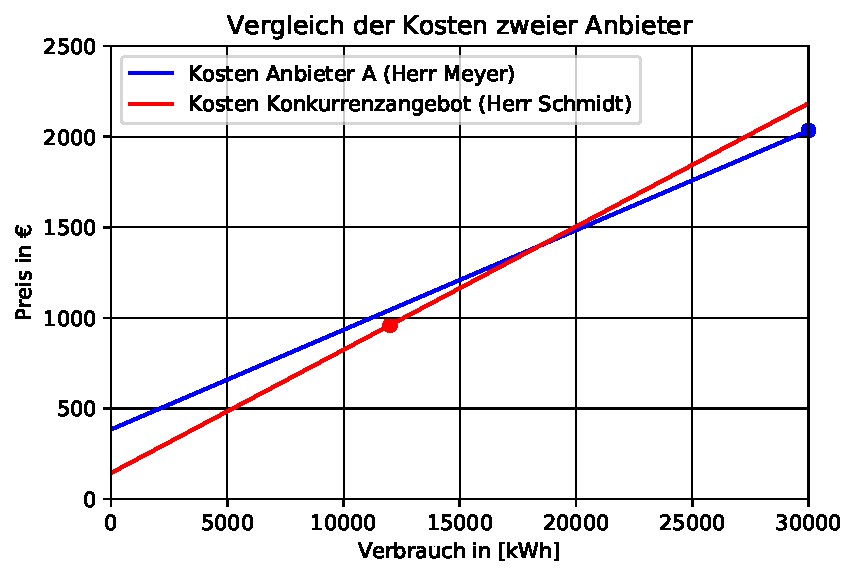
\includegraphics{Beispiel_1.pdf}
\caption{Bild 1: Beispieldiagramm}
\end{figure}


\end{document}


%%% Local Variables: 
%%% mode: latex
%%% TeX-master: t
%%% End: 
